\documentclass[tikz,border=4pt]{standalone}
\usepackage[T1]{fontenc}\usepackage[utf8]{inputenc}\usepackage{helvet}\renewcommand{\familydefault}{\sfdefault}
\begin{document}
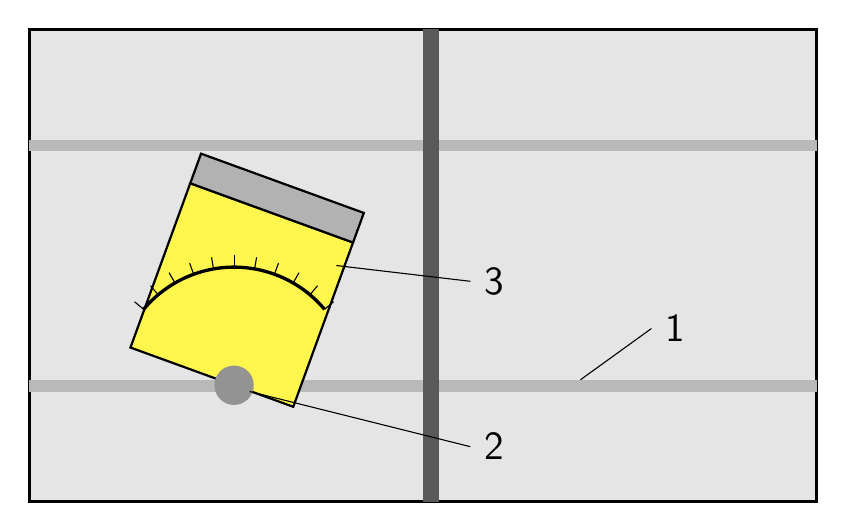
\begin{tikzpicture}[font=\Large]
% Sägetisch Draufsicht
\fill[gray!20] (0,0) rectangle (10,6); \draw[very thick] (0,0) rectangle (10,6);
% Führungsnuten
\fill[gray!55] (0,1.4) rectangle (10,1.55); \fill[gray!55] (0,4.45) rectangle (10,4.6);
% Sägeblattschlitz
\fill[black!65] (5.0,0) rectangle (5.2,6);
% Winkelanschlag: Anschlagleiste, drehbar um Mittelpunkt
\begin{scope}[rotate around={-20:(2.6,1.48)}]
 \fill[yellow!70] (1.2,1.48) rectangle (3.4,3.7); \draw[thick] (1.2,1.48) rectangle (3.4,3.7);
 \fill[gray!60] (1.2,3.7) rectangle (3.4,4.1); \draw[thick] (1.2,3.7) rectangle (3.4,4.1); % Anschlag
\end{scope}
% Skala 3 + Schraube 2 + Führung 1
\draw[very thick] (2.6,1.48) ++(40:1.5) arc (40:140:1.5);
\foreach \a in {40,50,...,140}{\draw (2.6,1.48) ++(\a:1.5) -- ++(\a:0.15);}
\fill[gray!85] (2.6,1.48) circle (0.25);
\node at (5.9,2.8) {3}; \draw (5.6,2.8) -- (3.9,3.0);
\node at (5.9,0.7) {2}; \draw (5.6,0.7) -- (2.8,1.4);
\node at (8.2,2.2) {1}; \draw (7.9,2.2) -- (7.0,1.55);
\end{tikzpicture}
\end{document}
